\documentclass[12pt,a4paper]{article}

\usepackage[utf8]{inputenc}
\usepackage[T1]{fontenc}
\usepackage[brazilian]{babel}
\usepackage{amsmath}
\usepackage{graphicx}
\usepackage{geometry}
\usepackage{float}
\usepackage{hyperref}

\geometry{top=2.5cm, bottom=2.5cm, left=3cm, right=3cm}

\title{Atividade: Algoritmo Perceptron \\ \large Disciplina: Redes Neurais Artificiais}
\author{Programa de Pós-Graduação em Ciência da Computação (PPGCC-UNESP)}
\date{\today}

\begin{document}

\maketitle

\section{Introdução}
Este documento apresenta os resultados da implementação e avaliação do modelo Perceptron original. Diferente do ADALINE, o Perceptron utiliza a saída discreta (após a função de ativação sinal) para calcular o erro. A atualização dos pesos ocorre apenas quando há um erro de classificação, seguindo a regra:
$$w^{atual} = w^{anterior} + \eta \cdot (d^{(k)} - y) \cdot x^{(k)}$$
onde $y$ é a previsão discreta ($1$ ou $-1$). Como o Perceptron não minimiza uma função de custo contínua, ele é conhecido por não convergir caso os dados não sejam linearmente separáveis, mantendo seus pesos em constante oscilação.

\section{Experimentos: Dataset 1}
O primeiro experimento foi conduzido em uma base de 2 atributos. Os parâmetros utilizados foram: limite de 100 épocas e taxa de aprendizado $\eta = 0.1$.

\subsection{Resultados Numéricos}
\begin{table}[H]
\centering
\begin{tabular}{|c|c|c|c|c|}
\hline
\textbf{LR ($\eta$)} & \textbf{Máx. Épocas} & \textbf{Épocas Executadas} & \textbf{Acc Treino} & \textbf{Acc Teste} \\ \hline
0.1 & 100 & 100 & 96.43\% & 95.00\% \\ \hline
\end{tabular}
\caption{Resultados obtidos para o Dataset 1}
\end{table}

\begin{figure}[H]
    \centering
    \begin{minipage}{0.48\textwidth}
        \centering
        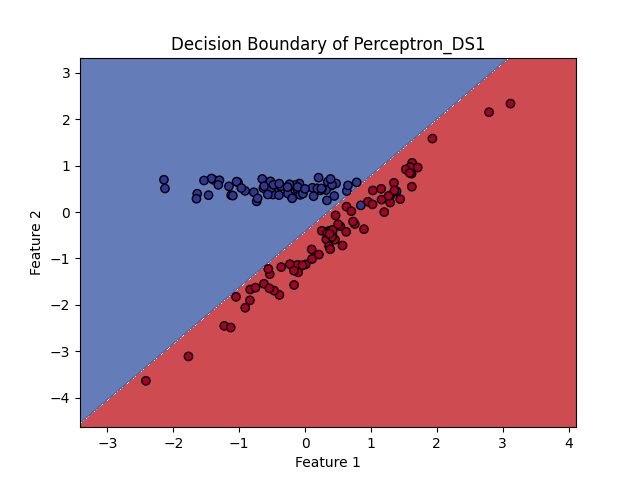
\includegraphics[width=\linewidth]{../../assets/perceptron/train_decision_boundary_Perceptron_DS1.png}
        \caption{Fronteira Treino (DS1)}
    \end{minipage}\hfill
    \begin{minipage}{0.48\textwidth}
        \centering
        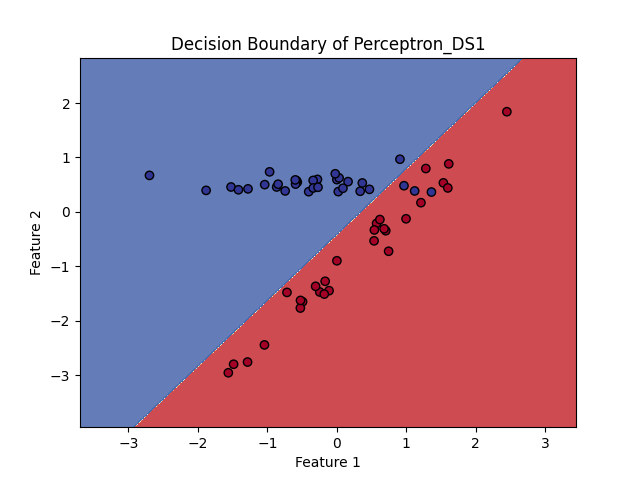
\includegraphics[width=\linewidth]{../../assets/perceptron/test_decision_boundary_Perceptron_DS1.png}
        \caption{Fronteira Teste (DS1)}
    \end{minipage}
\end{figure}

\textbf{Discussão (Dataset 1):} O modelo obteve um desempenho excelente neste conjunto de dados, atingindo 96.43\% de acerto no treino e 95.00\% no teste. Embora tenha executado todas as 100 épocas (indicando que restaram alguns pontos que impediram o erro zero absoluto), a altíssima acurácia demonstra que o Dataset 1 é quase perfeitamente separável de forma linear.


\section{Experimentos: Dataset 2}
O segundo experimento utilizou uma base de 2 atributos mantendo os mesmos hiperparâmetros ($\eta = 0.1$, máx 100 épocas).

\subsection{Resultados Numéricos}
\begin{table}[H]
\centering
\begin{tabular}{|c|c|c|c|c|}
\hline
\textbf{LR ($\eta$)} & \textbf{Máx. Épocas} & \textbf{Épocas Executadas} & \textbf{Acc Treino} & \textbf{Acc Teste} \\ \hline
0.1 & 100 & 100 & 42.86\% & 49.33\% \\ \hline
\end{tabular}
\caption{Resultados obtidos para o Dataset 2}
\end{table}

\begin{figure}[H]
    \centering
    \begin{minipage}{0.48\textwidth}
        \centering
        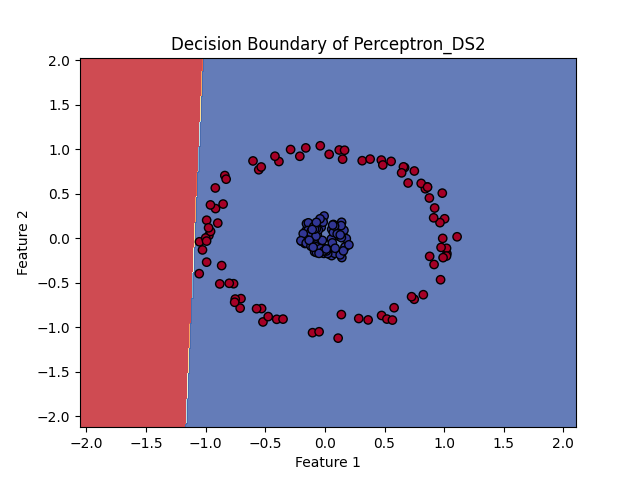
\includegraphics[width=\linewidth]{../../assets/perceptron/train_decision_boundary_Perceptron_DS2.png}
        \caption{Fronteira Treino (DS2)}
    \end{minipage}\hfill
    \begin{minipage}{0.48\textwidth}
        \centering
        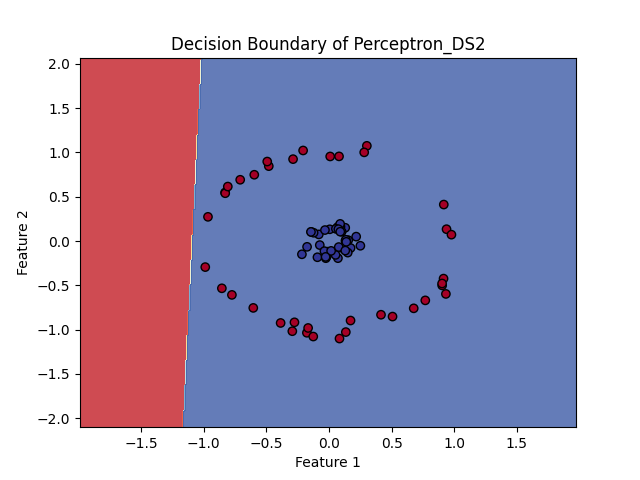
\includegraphics[width=\linewidth]{../../assets/perceptron/test_decision_boundary_Perceptron_DS2.png}
        \caption{Fronteira Teste (DS2)}
    \end{minipage}
\end{figure}

\textbf{Discussão (Dataset 2):} Os resultados no Dataset 2 ilustram a principal fraqueza teórica do algoritmo Perceptron. A acurácia despencou para cerca de 42.86\% no treinamento e 49.33\% no teste (um desempenho similar a um chute aleatório). Como os dados não são linearmente separáveis, a reta de decisão oscila infinitamente a cada época, tentando corrigir os erros de uma classe e fatalmente desclassificando a outra. Como o Perceptron não possui um mecanismo (como a margem suave do SVM ou o erro contínuo do Adaline) para "aceitar" o erro e parar em um mínimo global, ele simplesmente entrega o vetor de pesos da última iteração, que pode ser completamente subótimo.


\section{Experimentos: Dataset 3}
O Dataset 3 apresenta maior complexidade (alta dimensionalidade). Foram avaliadas múltiplas combinações de taxa de aprendizado ($\eta \in \{0.1, 0.001, 0.0001\}$) e número máximo de épocas ($100$ e $200$). A visualização gráfica da fronteira de decisão foi omitida devido à dimensão ($D > 3$).

\subsection{Comparativo de Hiperparâmetros}
\begin{table}[H]
\centering
\begin{tabular}{|c|c|c|c|c|}
\hline
\textbf{$\eta$} & \textbf{Máx. Épocas} & \textbf{Épocas Executadas} & \textbf{Acc Treino} & \textbf{Acc Teste} \\ \hline
0.1 & 100 & 100 & 87.76\% & 84.13\% \\ \hline
0.1 & 200 & 200 & 89.12\% & 80.95\% \\ \hline
0.001 & 100 & 100 & 93.88\% & 85.71\% \\ \hline
0.001 & 200 & 200 & 85.71\% & 87.30\% \\ \hline
0.0001 & 100 & 100 & 82.31\% & 74.60\% \\ \hline
0.0001 & 200 & 200 & 89.12\% & 82.54\% \\ \hline
\end{tabular}
\caption{Resultados do Perceptron no Dataset 3}
\end{table}

\textbf{Discussão (Dataset 3):} No Dataset 3, observa-se claramente o efeito da "dança" do hiperplano (oscilação) devido à complexidade do espaço de atributos e possíveis ruídos não separáveis linearmente. 
\begin{itemize}
    \item Com $\eta = 0.1$, aumentar de 100 para 200 épocas melhorou o treino, mas piorou o teste, indicando \textit{overfitting} sobre os dados ruidosos.
    \item A melhor estabilidade geral foi encontrada com $\eta = 0.001$. Em 100 épocas, ele atingiu a melhor acurácia de treino da tabela (93.88\%). Contudo, deixá-lo rodar até 200 épocas causou uma queda no treino (85.71\%) mas um aumento no teste (87.30\%). Isso comprova que os pesos não estão convergindo, mas sim saltando entre diferentes estados a cada época.
    \item Com $\eta = 0.0001$, a taxa de atualização foi demasiadamente pequena. Em 100 épocas, o modelo ainda estava "caminhando" em direção à solução (74.60\% no teste), precisando de 200 épocas para alcançar resultados compatíveis com os outros testes (82.54\%).
\end{itemize}
De maneira geral, o Perceptron apresentou uma capacidade decente de classificação em alta dimensionalidade, mas sua incapacidade de estabilizar os pesos em um ponto ótimo local (problema parcialmente resolvido pelo Adaline) torna seus resultados finais altamente dependentes da época exata de parada.

\end{document}
